\section{Auswertung}
\label{sec:Auswertung}

Alle in der Auswertung benutzten Mittelwerte werden über die Gleichung
\begin{equation}
\tilde{x}=\frac{1}{n}\sum_{i=1}^n {x_i}
\end{equation}
bestimmt. Die Standardabweichung der Mittelwerte ergibt sich zu 
\begin{equation}
\Delta{\tilde{x}}=\sqrt{\frac{1}{n(n-1)}\sum_{i=1}^n {(x_i-\tilde{x})²}}.
\end{equation}
Wird eine Größe bestimmt, welche sich aus fehlerbehafteten Daten zusammensetzt, ergibt sich der absolute Fehler über die \textsc{Gauss}schen Fehlerfortpflanzung 
\begin{equation}
\Delta{f}(x_1,..,x_n)=\sqrt{\left(\frac{\mathup{d}f}{\mathup{d}x_1}\Delta{x_1}\right)²+..+\left(\frac{\mathup{d}f}{\mathup{d}x_n}\Delta{x_n}\right)²}.
\end{equation}
Zur Berechnung aller Größen werden die nicht gerundeten Größen benutzt um Rundungsfehler zu vermeiden. Am Ende der Auswertung aller Größen werden diese auf die erste signifikante Stelle des Fehlers gerundet. 

\subsection{Bestimmung der Gitterkonstanten $g$}
Die gemessenen Winkel entstehen durch Beugung des Lichtes an einem Reflexionsgitter. Für die weitere Auswertung wird daher die Gitterkonstante $g$ benötigt. Dazu wird das bekannte Spektrum einer Quecksilberdampflampe untersucht. 
\begin{table}
\centering
\begin{tabular}{S S S[table-format=3.1] S[table-format=3.1] }
\toprule
\multicolumn{2}{c}{Spektrallinie} & \multicolumn{1}{c}{Wellenlänge}&\multicolumn{1}{c}{Winkel}\\
{Intensität} & {Farbe} & {$\lambda\:/\si{\nano\meter}$} & {$\tilde{\varphi}\:/\si{\degree}$}\\
\midrule
\text{stark}   & \text{gelb}    & 579.1 & 279.6\\
\text{stark}   & \text{gelb}    & 577.0 & 279.9\\
\text{stark}   & \text{grün}    & 546.1 & 282.0\\
\text{schwach} & \text{blaugrün}& 491.6 & 285.7\\
\text{stark}   & \text{violett} & 435.8 & 289.5\\
\text{schwach} & \text{violett} & 434.7 & 289.7\\
\text{stark}   & \text{violett} & 407.8 & 291.5\\
\text{stark}   & \text{violett} & 404.7 & 291.7\\
\bottomrule
\end{tabular}
\caption{Wellenlängen und Winkel der ausgemessenen Spektrallinien.}
\label{tab:hgspektrum}
\end{table}


In Tabelle \ref{tab:hgspektrum} sind die Winkel $\tilde{\varphi}$ aufgetragen, unter denen die verschiedenen Spektrallinien auftreten. Zur Bestimmung der tatsächlichen Beugungswinkel müssen einige Korrekturen durchgeführt werden. Alle Winkel sind relativ zur Position des nullten Maximums bei $\varphi_0=323,6\,\si\degree$ gemessen. Daher muss die Differenz $\tilde{\varphi}-\varphi_0=\varphi_\mathup{diff.}$ gebildet werden. Hinzu kommt, dass einlaufender und reflektierter Strahl anders als beim Transmissionsgitter einen Winkel von $2\beta=90\,\si\degree$ einschließen. Für die wirklichen Beugungswinkel $\varphi$ gilt also $\varphi=\varphi_\mathup{diff.}-\beta$.
Dargestellt wird der geometrische Zusammenhang in Abbildung \ref{fig:winkelbeziehungen}.
\begin{figure}
	\centering
	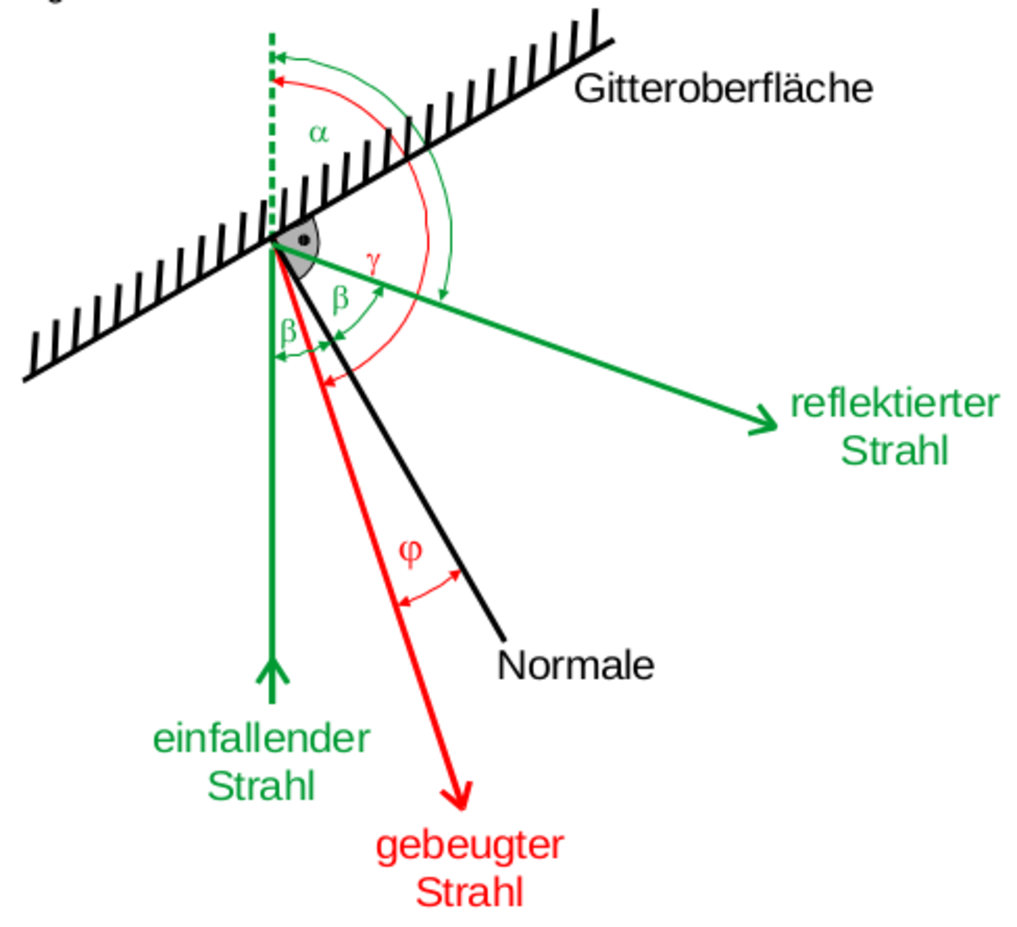
\includegraphics[width=0.5\textwidth]{Bilder/Winkelbeziehungen.pdf}
	\caption{Winkelbeziehungen bei Verwendung eines Reflexionsgitters.}\cite{skript}
	\label{fig:winkelbeziehungen}
\end{figure}
Um die Gitterkonstante $g$ zu bestimmen wird nach Gleichung \eqref{eq:hauptmaxima} $\sin{\beta}+\sin{\varphi}$ in Abhängigkeit von der Wellenlänge $\lambda$ aufgetragen. Es gilt
\begin{equation}
\sin{\beta}+\sin{\varphi}=\frac{\lambda}{g}.
\end{equation}
\begin{table}
\centering
\begin{tabular}{S S S[table-format=3.1] S[table-format=3.1] S[table-format=1.3] }
\toprule
{$\varphi\:/\si{\degree}$} & {$sin(\varphi)$}\\
\midrule
 -0.017 & -0.0175\\
 -0.023 & -0.0227\\
 -0.059 & -0.0593\\
 -0.124 & -0.1239\\
 -0.190 & -0.1902\\
 -0.194 & -0.1937\\
 -0.225 & -0.2251\\
 -0.229 & -0.2286\\
\bottomrule
\end{tabular}
\caption{Korrigierte und zur Rechnung benötigte Winkel der Spektrallinien.}
\label{tab:2}
\end{table}
Daraus ergibt sich mit den Werten aus Tabelle \ref{tab:2} und linearer Regression eine Geradengleichung
\begin{equation}
f(x)= \underbrace{(0.001192 \pm 0.000006)\,\frac{1}{\si{\nano\meter}}}_{Steigung\,\triangleq\,\sfrac{1}{g}}x-(0.002 \pm 0.003),
\label{eq:lin_reg}
\end{equation}
deren reziproke Steigung dem Wert der Gitterkonstanten
\begin{equation}
g=(839 \pm 3)\,\si{\nano\meter}
\label{eq:gitterkonst}
\end{equation}
entspricht.
\begin{figure}
	\centering
	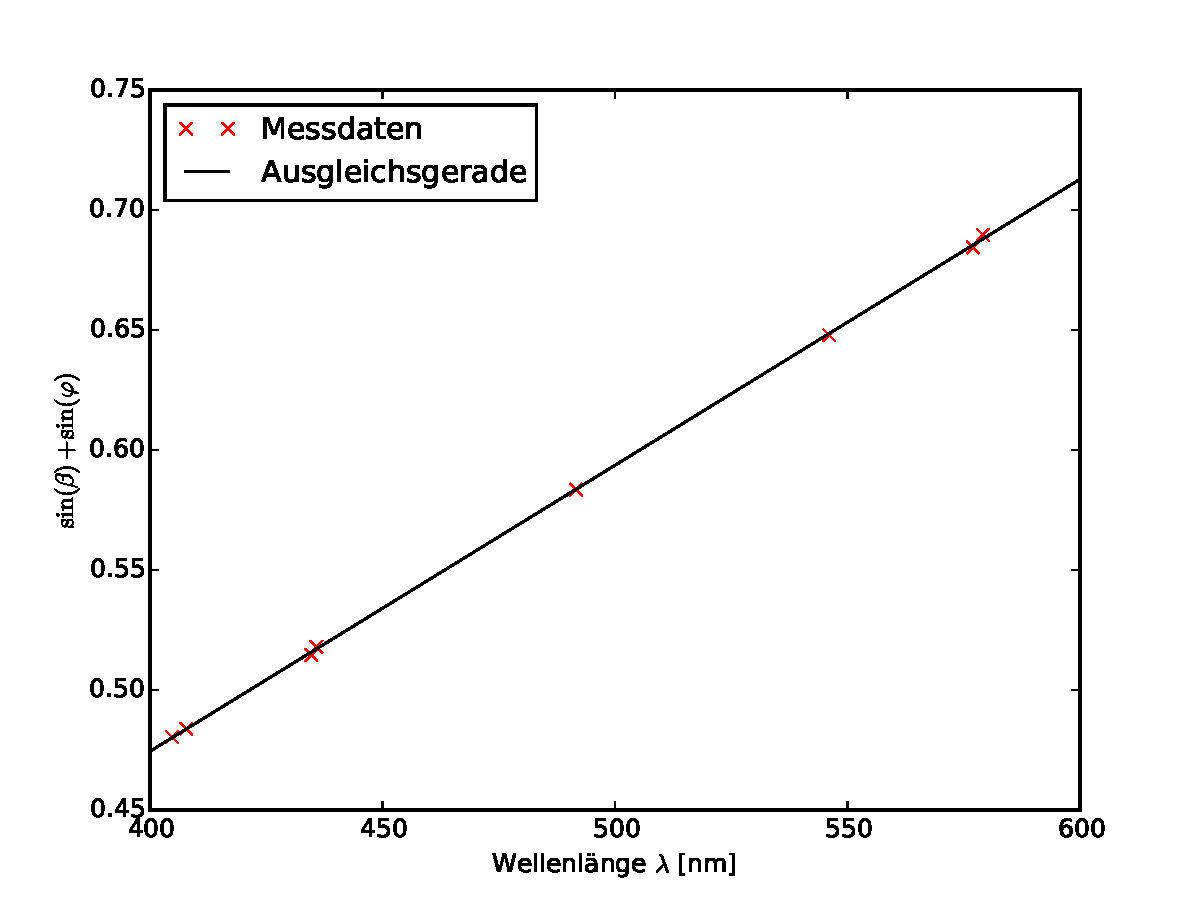
\includegraphics[width=\textwidth]{Bilder/Gitterkonstante.pdf}
	\caption{Lineare Regression zur Bestimmung von $g$.\cite{skript}}
	\label{fig:lin_reg}
\end{figure}
\subsection{Untersuchung der Alkalispektren}
Es werden die Spektren einer Natrium-\footnote{\Bat}, Kalium - und Rubidiumdampflampe ausgemessen. Nähere Betrachtung erfahren hier die Dublett-Linien. Die beobachteten Linien entstehen durch aufspalten des 3P-Niveaus bei Natrium, des 4P-Niveaus bei Kalium und des 5P-Niveaus bei Rubidium.  Da die Dubletts sehr nahe beieinanderliegen wird zur Abstandsmessung ein Okularmikrometer benutzt. Dieses wird zuvor geeicht. $143$ Skalenteile entsprechen einer Winkeländerung von $\SI{0,3}{\degree}$. Damit kann der Eichfaktor zu $\gamma=0.015\,\si{\nano\meter}\,/\text{Skt.}$ berechnet werden. 
\begin{table}
\centering
\begin{tabular}{S  S[table-format=3.1] S[table-format=1.4] S[table-format=3.1] S[table-format=1.0(1)] S[table-format=1.0] S[table-format=1.3(1)] S[table-format=1.5(1)] }
\toprule
%\multicolumn{2}{c}{Spektrallinie} & \multicolumn{1}{c}{Wellenlänge}&\multicolumn{1}{c}{Winkel}\\
{Element} & {$\tilde{\varphi}\:/\si\degree$} & {$\varphi\:/\si\degree$} & {$\mathup{\Delta{s}}\:/\mathup{Skt.}$}& {$\lambda\:/\si{\nano\meter}$} & {$\Delta{\lambda}\:/\si{\nano\meter}$}&{$\Delta{E}\:/\si{\milli}\mathup{e}\si\volt$}&{$\sigma$}\\
\midrule
\text{Na}  & 277.1 &  0.0262 &  50.0 & 615(3) & 0.73 &  2.41(2)    &   7.34066(6)  \\
           & 278.9 & -0.0052 &   4.8 & 589(3) & 0.70 &  0.252(2)   &   8.91784(4)  \\
           & 280.3 & -0.0297 &   3.7 & 568(3) & 0.05 &  0.209(2)   &   9.01436(3)  \\
\text{Ka}  & 279.8 & -0.0209 & 128.0 & 576(3) & 1.88 &  7.03(7)    &  13.0625(1)    \\
           & 279.9 & -0.0227 & 158.0 & 575(3) & 2.32 &  8.73(8)    &  12.7337(1)  \\
           & 283.0 & -0.0768 & 113.0 & 529(2) & 1.65 &  7.34(7)    &  12.9996(1)  \\
           & 283.3 & -0.0820 & 100.0 & 525(2) & 1.46 &  6.60(6)    &  13.1565(1)    \\
\text{Rb}  & 276.4 &  0.0384 & 656.0 & 625(3) & 9.63 & 30.5(3)     &  26.8692 (2)   \\
\bottomrule
\end{tabular}
\caption{Gemessene, sowie berechnete Werte der Alkali-Spektren.}
\label{tab:spektren}
\end{table}
In Tabelle \ref{tab:spektren} werden die aufgenommenen, sowie um $\varphi_0$ und $\beta$ korrigierten Wete gelistet. Der Winkel $\varphi$, unter welchem die Liniendubletts zu sehen sind, wird durch Mittelwertsbildung der Winkel beider Linien ermittelt. Zwischen den Linien liegt eine Entfernung $\mathup{\Delta{s}}$ . Die Wellenlänge $\lambda$, sowie der Wellenlängenunterschied $\mathup{\Delta{\lambda}}$ werden nach Gleichung \eqref{delta_lambda} berechnet. Mit Gleichung \eqref{delta_E} kann nun die Energiedifferenz $\mathup{\Delta{E}}$ und damit die Abschirmungszahl $\sigma$ bestimmt werden.
Die Abschirmungszahlen ergeben sich mit den Werten aus Tabelle \ref{tab:spektren} zu 
\begin{align}
\sigma_\mathup{Na}&=\SI{8.424285(3)}{}, \\
\sigma_\mathup{K\:}&=\SI{12.988059(5)}{},\\
\sigma_\mathup{Rb}&=\SI{26.8692(2)}{}.
\end{align}
